%! TEX root = ./main.tex

\lecture{12}{Week 6}{Compiling C Data Structure}

This chapter is important because it tells us what happens in memory.

\subsubsection{Recap: Basic Data Types}
The fundamental data types on C are integers and floating-point values. They are both stored and operated on in dedicated integer respectively floating point registers. For integers, we differentiate between signed and unsigned and the interpretation depends on the used instruction.

The following table summarizes their size:

\begin{tabular}{l l l l}
    Intel & GAS & Bytes & C\\
    \hline
    byte & n & $1$ & signed/unsigned char\\
    word & w & $2$ & signed/unsigned short\\
    double word & l & $4$ & signed/unsigned int\\
    quad word & q & $8$ & signed/unsigned long int (x86-64)\\
    \hline
    single & s & $4$ & float\\
    double & l & $8$ & double\\
    extended & t & $10/12/16$ & long double\\
\end{tabular}

\textit{GAS} stands for Gnu Assembly Format.

Pointers used to be $4$ bytes long on ia32, on x86-64 they are $8$ bytes long.

\subsubsection{Arrays}
\paragraph{One-Dimensional Arrays}
One dimension arrays are blocks of homogeneous data structured contiguously in memory. The type of data it contains, determines the size of a single element. The length of the array is the size of each single block times the length of the array.

Since there is no out-of-bounds check for array, we may access random data when indexing an element which is not part of the array. When we define multiple arrays, they may be placed contiguously in memory and this way we may access the second array via the pointer of the first array. However, this is not guaranteed to works and hence, should be omitted. Compiler may arrange data in memory however they like. Compiler may also notice out-of-bound accesses and remove such instructions.

When iterating over an array and accessing its elements, compiles may eliminate loop variables and instead use pointers.

\paragraph{Nested Arrays}
Nested arrays are multidimensional arrays. Since C is row-major, row elements are stored contiguously and all the single rows itself again.

They are declared as \code{T A[R][C];} and in this example, the array would be $2$D and contains R rows and C columns. Hence, the array would be of size \code{R * C * sizeof(T)}.

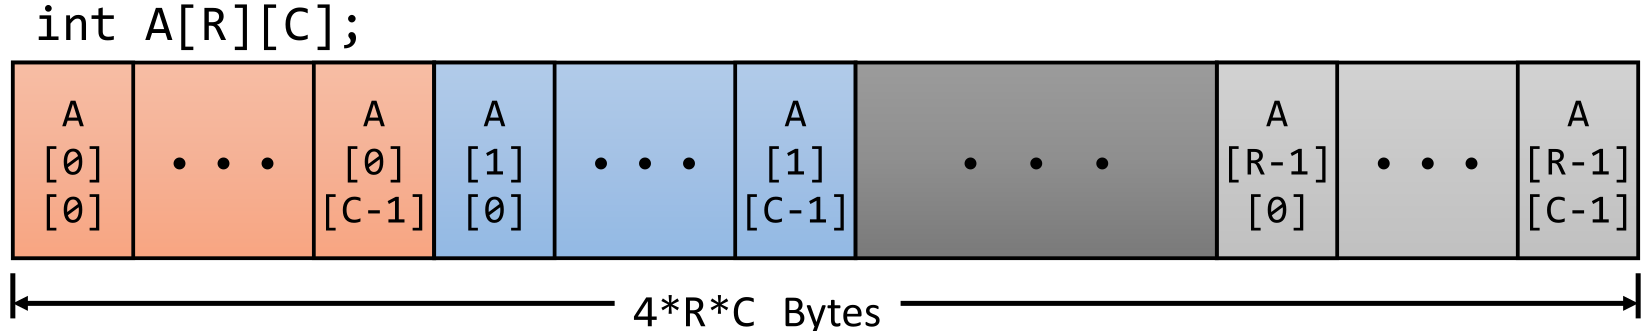
\includegraphics[width=1\textwidth]{12_nestedArrays.png}

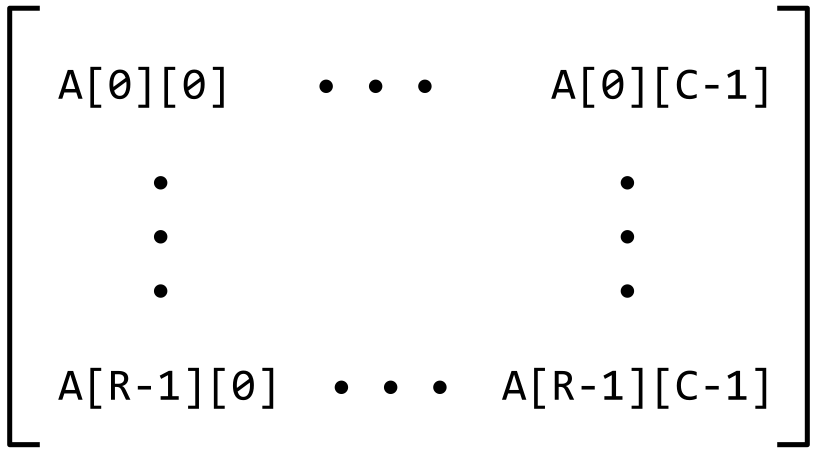
\includegraphics[width=0.8\textwidth]{12_nestedArrayStructure.png}

Since all rows are arranged contiguously, it is guaranteed that we can index into other rows. The access of any element, e.g. \code{<row>, <column>} is possible with only one memory access with the formula $base\_addr + row * column\_len * sizeof(T) + column * sizeof(T) = base\_addr + (row * column\_len + column) * sizeof(T)$.

However, there can be \textit{weird} cases where this is not guaranteed (not exam relevant...).

\paragraph{Multi Level Array}
Multi level arrays are constructed of several separate arrays. It is actually rather an array of pointers to array and it is also declared as \code{int *A[R]}. So, the rows of the array are not guaranteed to be placed contiguously in memory and therefore, one cannot access any element of the array by adding an offset to the base pointer. But instead, we have to first access the \textit{pointer array}, and then access the desired element. This requires two memory accesses compared to only one for nested arrays. For arrays of higher dimension, even more memory accesses are required.

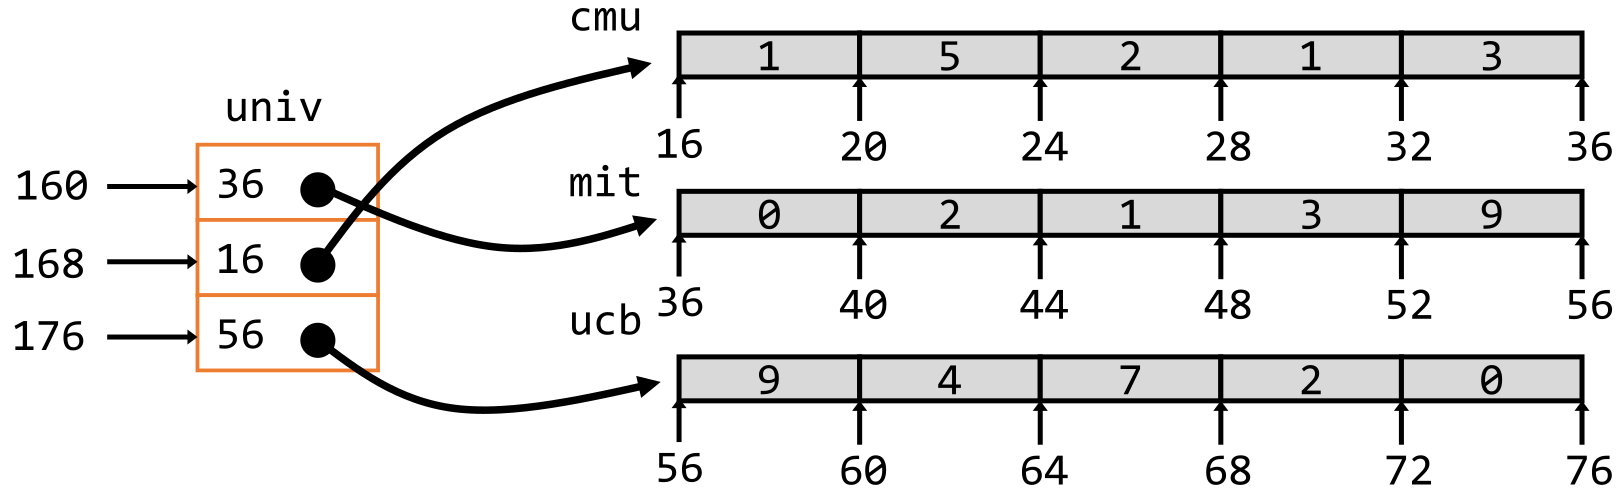
\includegraphics[width=1\textwidth]{12_multilevelarrayoverview.png}

\paragraph{Arrays for Matrix Multiplication}
Compilers are good at doubly subscripted array accesses. However, in order to implement represent an matrix with nested arrays, its size needs to be known at compile time. When we want it more dynamically, we may implemented the \textit{nested array structure ourself} by heaving a block of memory and do all index computation by ourself. Since we need to do many multiplications and access of single elements are therefore rather costly, this is not very performant. Nevertheless, compiler are actually quite good at improving this solution since there are many regular patters for e.g. a matrix multiplication.

\subsubsection{Structures}
Stucts are a contiguously-allocated region of memory. The values are ordered contiguously in the same order as their are defined. Since they are arrange contiguously, we can theoretically access a subsequent element via the address of a previous element.

\paragraph{Alignment}
For performance reasons, data is always aligned in memory. If it ways not, maybe multiple memory accesses may be required to read or write instead of just one, because memory is accessed in junks of $4$ or $8$ bytes (system dependant).

For x86-64 we have to following alignment cases:
\begin{description}
    \item[1 byte:] char
    \item[2 bytes:] short
        \begin{itemize}
            \item lowest $1$ bit of address must be $0_2$
        \end{itemize}
    \item[4 bytes:] int, float
        \begin{itemize}
            \item lowest $2$ bits of address must be $00_2$
        \end{itemize}
    \item[8 bytes:] double, char, *
        \begin{itemize}
            \item lowest $3$ bits of address must be $000_2$
        \end{itemize}
    \item[16 bytes:] long double
        \begin{itemize}
            \item lowest $3$ bits of address must be $000_2$ (treated equivalently to $8$ byte aligned types)
        \end{itemize}
\end{description}

In short this means that if a primitive data type requires $K$ bytes, it is always aligned on a multiple of $K$.

In order that the data fields in the strut are aligned, the compiler may add padding between fields. Therefore, it is also not guaranteed that we can access a subsequent field by simple adding some padding. The placement of the struct itself is determined by the sizes of its fields. If $K$ is the alignment of the largest field, then the struct is aligned at a multiple of $K$.

It may be optimal to define files of larger types first, but since the whole struct must be aligned in a multiple of the size of the largest fields, in practice there is not much gain.

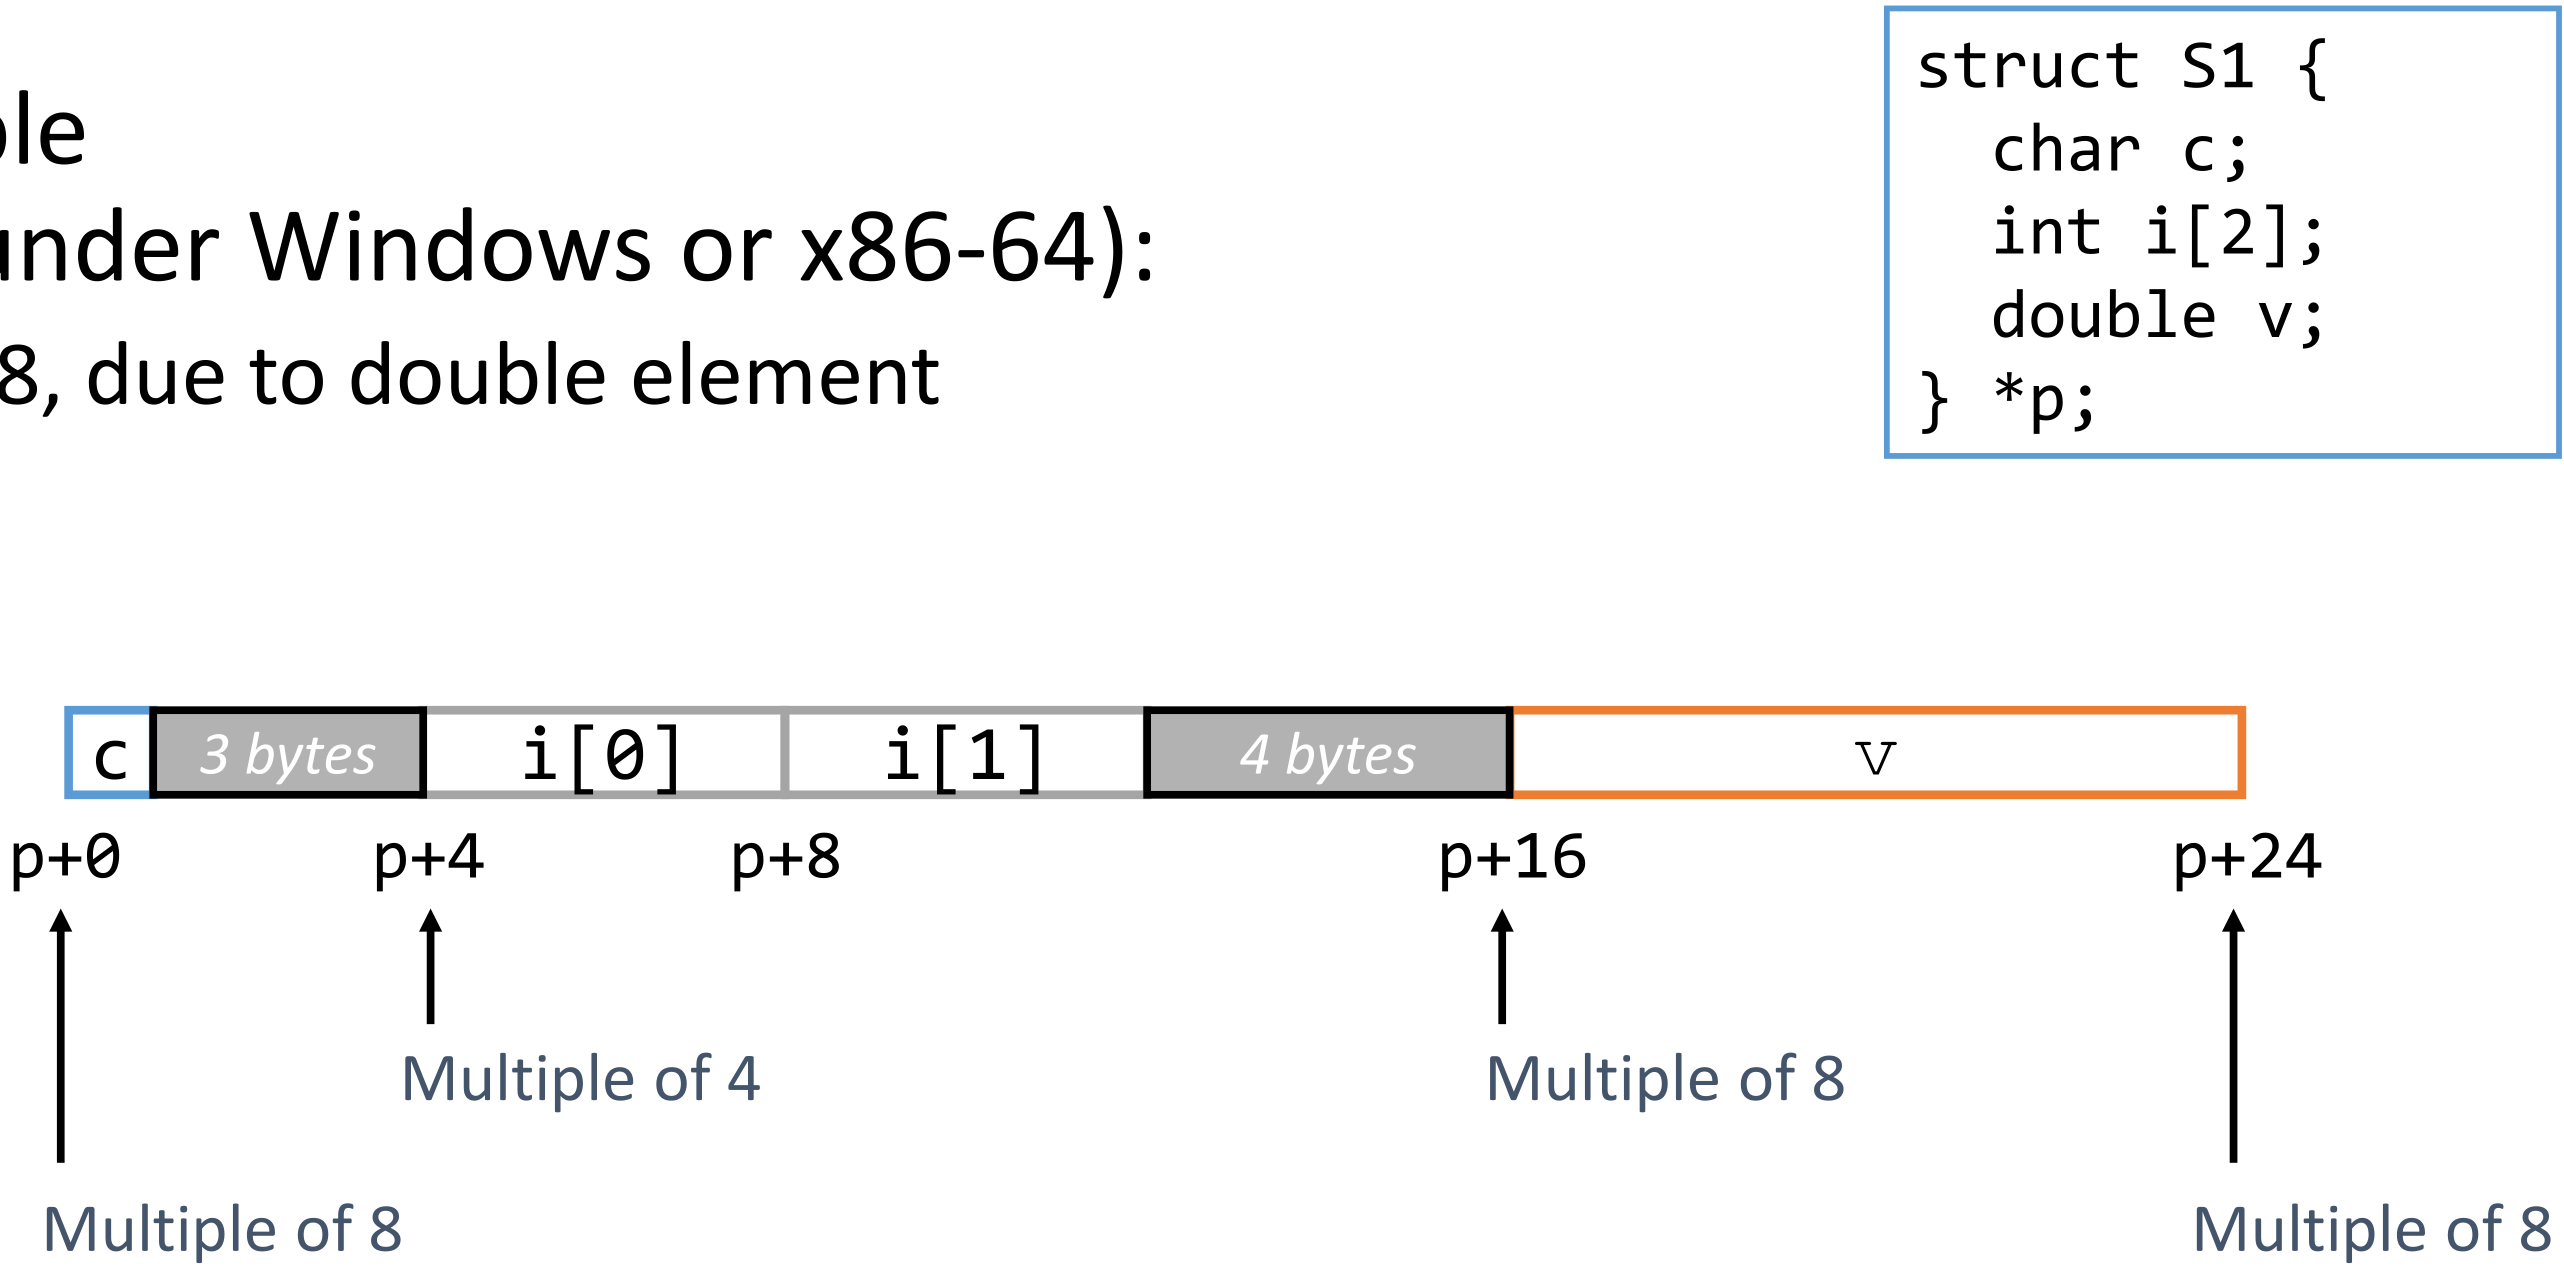
\includegraphics[width=0.8\textwidth]{12_structAlignment.png}

\paragraph{Arrays of Structures}
Stucts in arrays have to follow the alignment requirements too. This may lead to lots of unused padding space.

\subsubsection{Union}
The size of a union is simply the size of the largest field. The space for the fields is \textit{overlayed}.

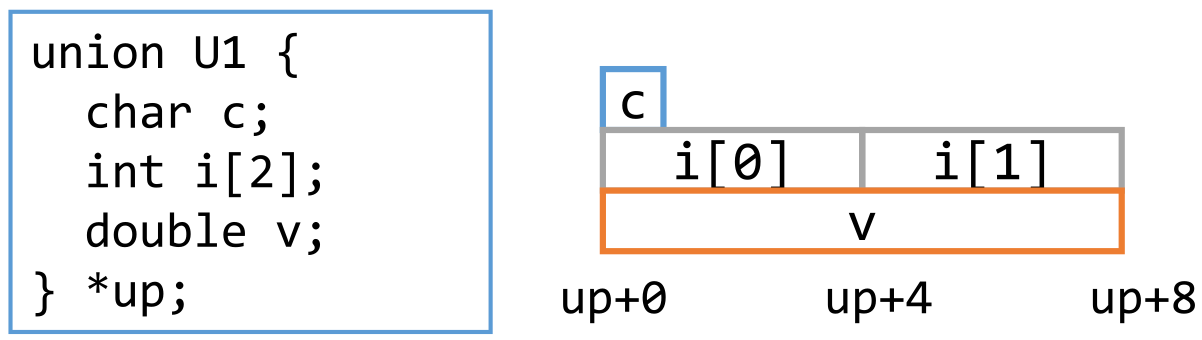
\includegraphics[width=0.8\textwidth]{12_union.png}
